\documentclass{beamer}
\usepackage[UTF8,noindent]{ctexcap}
\usepackage{beamerthemesplit}  
\usepackage{amsmath}
\usetheme{Berlin}
\newtheorem{formula}{公式}

\title{基于JESD204B的Serdes接口中接受电路设计研究}
\subtitle{开题报告}
\author{陈登 \\导师:姚亚峰}
\date{\today}
\begin{document}

\begin{frame}
	\titlepage
\end{frame}

\begin{frame}{目录}
	\tableofcontents
\end{frame}

\section{选题依据}

\begin{frame}{选题依据}{SERDES接口介绍}
在通信系统中,尤其是无线通信系统,高速AD转换芯片的地位非常重要。伴随着通信系统的传输速率不断飞速增长,传统的AD数据接口,如USB、SPI、I2C,已经远远无法满足在更高速条件下信号传输的需求。于是一种新的接口技术,SERDES应运而生,逐渐成为高速AD芯片上的必备接口,在实际中有着广泛的应用。
\end{frame}

\begin{frame}{选题依据}{选题意义}
本设计着重需要完成的是基于JESD204B协议标准,设计出适用于高速AD、DA转换芯片的SERDES接口接收端电路。主要包括数据链路层和传输层的逻辑设计、差错控制等。

由于JESD204B协议是JESD的一个较新的适用于SERDES接口的协议,相较于前两版本的协议在数据链路层、传输层都有一定的改动,增加了其使用灵活性,并且新协议版本向下支持以往的协议。正因为其发布时间不长,相关的设计和实现比较缺乏,所以主要的难点在于对新协议的理解和掌握,能够跟上时代的步伐。
\end{frame}

\begin{frame}{选题依据}{国内外研究现状及发展趋势}
SERDES接口芯片在数据传输中体现出来的一系列优点,已经引起了国内外研究机构和产业界的重视。目前国内以复旦大学、东南大学、国防科技大学为代表的研究机构已经对SERDES技术进行了一系列研究,也取得了丰硕的研究成果。在产业界,国外的Lattice公司于2009年推出内嵌SERDES的FPGA产品。德州仪器公司也开发出了系列SERDES接口芯片,如 TLK2711A、TLK3101、TLK4120 等等。虽然目前串行通信主流的应用是传输速率在1Gb/s到10Gb/s之间的应用,但是业界一直朝着不断提高传输速率的方向努力,安华高科技于2008 年首次在40nm CMOS工艺上实现20Gbps的SERDES。
\end{frame}

\begin{frame}{选题依据}{存在的问题}
现在国内市场上还很少能够看到自主生产的、拥有知识产权的、带有SERDES接口的AD、DA芯片。并且很多现有的芯片并没有采用最新的JESD204B协议。本课题研究的SERDES接口接收端电路能够实际应用成为完整SERDES接口的一部分,具有一定的价值。
\end{frame}

\section{研究内容和目标}

\begin{frame}{研究内容和目标}{研究内容}
	\begin{itemize}
	\item SERDES接收端数据链路层设计:8B/10B解码器设计,解扰器设计,同步检测设计,差错控制报错设计。
	\item SERDES接收端传输层设计:解帧器设计,差错报错控制设计。
	\item 外围电路设计:伪随机序列生成电路设计、测试电路设计。
	\end{itemize}
\end{frame}

\begin{frame}{研究内容和目标}{接收端系统框图}
	\begin{figure}
	\centering
	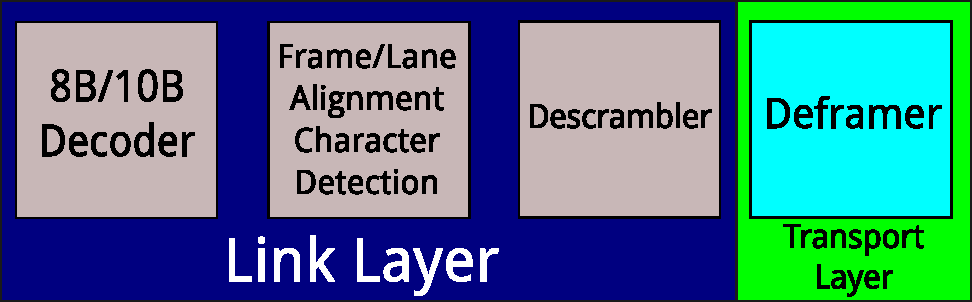
\includegraphics[scale=0.6]{serdes_sturct_link_transport_layer.pdf}
	\caption{接收端系统框图}
	\end{figure}
\end{frame}

\begin{frame}{研究内容和目标}{研究目标}
	\begin{itemize}
	\item 设计出符合JESD204B协议标准的SERDES接收端的数据链路层和传输层电路设计,完成RTL仿真及综合。
	\item 在SMIC 180nm工艺标准下,固定导线负载标准下。
		\begin{itemize}
		\item 整体工作频率达到500Mhz。
		\item 单元面积小于10000$\mu m^2$。
		\end{itemize}
	\item 能够通过配置寄存器调整传输模式、传输速度等,能够通过接口报告错误,具有一定的差错处理能力。
	\end{itemize}
\end{frame}

\begin{frame}{研究内容和目标}{拟解决关键问题}
为完成一个基于JESD204B协议的SERDES接收端电路设计,需要解决的关键技术有
	\begin{itemize}
	\item 数据链路层电路设计。根据设计需要,设计所需的各个子模块,如8B/10B解码器,解扰器,同步检测模块。
	\item 传输层电路设计。通过链路层获得的数据进一步将整合在一个包中的数据解开,对其中发生的错误进行纠正或报错。
	\item 通过最终的连接仿真,要达到正确传输的一般功能外,还要达到预期的技术指标。
	\end{itemize}
\end{frame}

\section{选题研究方案、可行性分析及特色}

\begin{frame}{选题研究方案、可行性分析及特色}{研究方法}
通过对已有研究成果和JESD204B协议的理解,分析以及对现存的各种SERDES接口电路设计的探索,力求使系统工作频率高,芯片面积小,功能达到预期要求,从数据链路层和传输层两个层面对课题进行设计研究。
\end{frame}

\begin{frame}{选题研究方案、可行性分析及特色}{技术路线}
基于JESD204B的Serdes接口中接收电路设计主要由输入信号的有数据链路层和传输层两个部分及测试部分构成。
	\begin{itemize}
	\item 数据链路层主要负责解码、解扰、同步等工作,重点在于对每个字节的处理。
	\item 传输层主要负责解帧的工作,重点在于对于一串字节的处理。
	\item 外围测试电路设计,主要为伪随机序列生成、输入信号生成,来模拟发送端的数据完成逻辑测试。
	\end{itemize}
\end{frame}

\begin{frame}{选题研究方案、可行性分析及特色}{实验方案}
	\begin{itemize}
	\item 通过Verdi3作为前期的设计Debug工具。
	\item 设计通过Modelsim的RTL级仿真来确保逻辑的工作正确。
	\item 设计复杂的testbench来完成可靠性的测试,依据协议规定还需要使用伪随机序列来对正确性进行测试。
	\item 完成RTL级仿真后再使用Design Compiler进行门级综合,使用SMIC 180nm工艺,固定导线负载,通过综合结果判断设计性能。
	\end{itemize}
\end{frame}

\begin{frame}{选题研究方案、可行性分析及特色}{特色}
	\begin{itemize}
	\item 本课题主要关注业界最新的JESD204B协议,其中含有新的数据链路层控制逻辑,并且要保证向下兼容。
	\item 电路设计层级提升到综合级别,相较于RTL级别的设计能更直观的判断电路的好坏,并且采用的是ASIC的设计思路,直接使用的是厂方工艺库,更贴合业界需求。
	\item 在保证面积和功耗的前提下,在特定的工艺级别下,能够达到较高的工作频率。
	\end{itemize}
\end{frame}

\section{学位论文工作计划及预期研究成果}

\begin{frame}{学位论文工作计划}{计划}
	\begin{description}
	\item[2014.11-2014.12] 协议理解、文献阅读
	\item[2014.12-2015.01] 数据链路层设计
	\item[2015.01-2015.02] 传输层设计
	\item[2015.02-2015.03] 数据链路层、传输层联调
	\item[2015.03-2015.05] 撰写论文
	\end{description}
\end{frame}

\end{document}